\section{Saturation in  Bipolar Junction Transistors}
\label{lab_bjt_saturation}

%\makelabheader %(Space for student name, etc., defined in master.tex)

\bigskip

\textit{In this lab, we'll look closely at the behavior of an npn bipolar junction transistor under different operating conditions, simultaneously measuring the voltage and current at all three transistor terminals.  Rather than trying to scrounge up six multimeters for the job, we'll simulate the transistor's behavior in Multisim instead.}

\begin{enumerate}[wide]

\item Build a model of the circuit shown below in Multisim.  Add voltage and current probes to all three leads of the transistor as shown.  By default, the probes will display both the AC and DC components of the signals; to display only the  DC values as shown below, click on the gear icon by the probe toolbox (``probe settings'') and select ``Instantaneous only.''  
\begin{center}
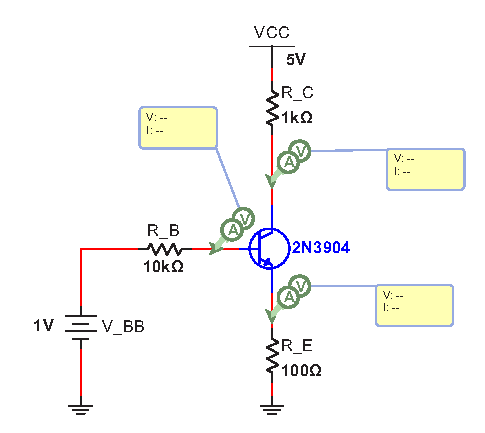
\includegraphics{bjt_saturation/bjt_saturation1.eps}
\index{color_page}
\end{center}

\item Run simulations of the circuit for values of the voltage source $V_{BB} = 0$, 1, 1.2, 1.5, 2, and 5 volts.  For each value of $V_{BB}$, record in a table the values of all six voltages and currents, and calculate the ratio of  $I_C/I_B$.

\item You learned in Lab~\ref{lab_bjt} that $I_C / I_B = h_{FE}$, where the constant value of $h_{FE}$ is about 150 for the 2N3904.  For what values of $V_{BB}$ in your table does $I_C/I_B$ have that approximate value?

\item You also learned in  Lab~\ref{lab_multisim} that the amplifier you designed only worked as you intended when $V_C > V_B > V_E$.  For what values of $V_{BB}$ in your table is that true?

\item In fact, bipolar junction transistors have three distinct ``modes of operation'' depending on the relative voltages of their terminals.  For an npn transistor,
\begin{itemize}[nosep]
\item $V_C > V_B \leq V_E$: ``cut-off mode'' (all currents $\approx 0$)\footnote{Some authors extend ``cut-off mode'' to include any $V_{BE} \lesssim 0.7$~V where $I_C \approx 0$.}
\item $V_C > V_B > V_E$: ``active mode''  (e.g. a working amplifier)
\item$V_C < V_B > V_E$: ``saturation mode''
\end{itemize}
Label each row of your data table to show which operating mode your transistor is in.

\item We say that a p-n junction is ``forward-biased'' when the p-type material is at a higher potential than the n-type material.  (For a regular single diode, current flows when it is forward biased.)  A junction is ``reverse-biased'' when the n-type material is at the higher potential.  For each of the three operating modes above, indicate whether the emitter-base junction is forward- or reverse-biased, and whether the collector-base junction is forward- or reverse-biased.  (Remember, the transistor you are using is an npn BJT.)

\item If you think about what's happening to $V_C$ as you raise $V_{BB}$, you'll realize that your single BJT transistor can be used as a simple inverter, or NOT gate, using $V_{BB}$ as the input and $V_C$ as the output.  (For this application, you can remove the resistor $R_E$ from your circuit, or just set its value to $R_E = 0$~$\Omega$.)  When you set the input to 0~V or 5~V, how close is the output to being exactly of 5~V or 0~V?  

\item Which operating mode is your transistor in when the inverter's output is high?  Which operating mode is it in when  the inverter's output is low?  

\item If you remove the resistor $R_B$ as well, you can increase the voltage $\Delta V_{BE}$ substantially beyond the nominal 0.7 volts.  However, when you do so, you'll pull a lot of current through the transistor, mostly from the base, and it will heat up like crazy.  Based on its size, about what should be the maximum power you can dissipate in a small transistor like the 2N3904?  Place a power probe directly on top of the 2N3904 to see how many Watts are dissipated in your transistor for various $V_B$.  (The icon for the power probe  is next to the voltage and current probes you've been using already; it's the little magnifying glass with a ``W'' inside for ``Watts''.)  What is the maximum value you can set for $V_B$ before the transistor would likely be ruined?


\end{enumerate}









